\documentclass[a4paper, 12pt]{article}
 % This is used for setting the margins
\usepackage[top=1in, bottom=1in, left=1in, right=1in]{geometry}

%%%% IMPORTED PACKAGES %%%
\usepackage{graphicx}
\usepackage{amsmath}
% Important when citations include URLs.
\usepackage[pdftex]{hyperref}
%%%%%%%%%%%%%%%%%%%%%%%%%%

\newenvironment{keywords}
{\begin{list}{}{\setlength{\leftmargin}{1em}}\item[\hskip\labelsep \bfseries Keywords:]}
{\end{list}}

\begin{document}

%%%%%%%% COVER %%%%%%%%%%%
\begin{titlepage}
\begin{center}
	\vspace{5 mm}
	    \textbf{\Large TECHNICAL UNIVERSITY OF MADRID}
	\par
	\vspace{10 mm}
	\begin{figure}[htb]
	    \centering
	    
\includegraphics[scale=0.7]{images/general/uni-logo.png}
	\end{figure}

    %\vspace{10 mm}\textbf{\large \degree} \par
    %\vspace{10 mm}\textbf{\large \faculty} \par
    %\vspace{20 mm}\textbf{\large \department } \par


    \vspace{20 mm}\textsc{\Large Analysis of Spanish COVID-19 tracking apps}
    \par
    \vspace{10 mm}\textsc{I\&E Seminars: Digital Health}
    \par
    \vspace{10 mm}
    \textsc{
        AUTHOR: \\
        Cristian M. Abrante Dorta
    }
    \par
	\rule{80mm}{0.1mm}\\
	\vspace{10 mm}
	
    \vspace*{\stretch{2}}
    \textsc{EIT Digital Master's degree in Data Science}\\
    \textsc{\today}
\end{center}
\end{titlepage}

%%%%%%%%%%%%%%%%%%%%%%%%%%

%%%%%% ABSTRACT %%%%%%%%%%
\newpage
\begin{abstract}
{\em

COVID-19 pandemic has affected the entire society on a deep level. Finding new solutions for fighting against it has been a really important coordinated effort between institutions, companies, and governments. The development of software applications could be a key aspect in the control of the spreading of the virus. In this survey, it is covered the current approaches followed for the development of applications regarding the pandemic. 

\bigskip

Also in this paper, it is discussed the case of Spain, where the impact of the pandemic and the decentralized nature of the healthcare system has conditioned the development of software solutions.
}

\begin{keywords}
COVID-19, Applications, Software, Pandemic tracking
\end{keywords}
\end{abstract}

\newpage{\pagestyle{empty}}
\thispagestyle{empty}

%%%%%%%%%%%%%%%%%%%%%%%%%%

%% TABLE OF CONTENTS %%%%%
\tableofcontents
\newpage{\pagestyle{empty}}

%%%%%%%%%%%%%%%%%%%%%%%%%%

%%% Set the counter of the page to 1 after the index.
\setcounter{page}{1}

%%%%%%%% INTRODUCTION %%%%%%%
\section{Introduction}
\label{section:introduction}

COVID-19 pandemic has caused a huge impact all over the world. The consequences of this pandemic are going to be cross-sectional, affecting both the economical development of many regions but also it is going to change the social behavior on a deep level. In this sense, also the healthcare systems have to be re-think and adapted for this new situation, taking into account that in the future this could happen again. \\

Mobile technology has been relevant to solving healthcare issues in the past. And as we keep our mobile devices with us all day long, they could be also really relevant for fighting the COVID-19 pandemic. Using this device as the development platform could be the key to controlling the dynamic environment of the pandemic, which evolves fast and in an exponential way. The objective of this survey is to cover the main approaches present nowadays for the development of software applications that could help health authorities to fight the pandemic. \\

In Section \ref{section:discussion}, we are going to focus on the concrete case of Spain. This country has been one of the most affected by the pandemic in the world, it was one of the epicenters of the illness at the beginning of March, and the government decreed strict lockdown measures in the middle of that month. The healthcare system in Spain is decentralized, where the majority of the competences on health issues correspond to the Autonomous Communities (\textit{Comunidades autónomas} in Spanish), which caused an uneven development of the illness in the different regions.

\begin{figure}[h]
    \centering
    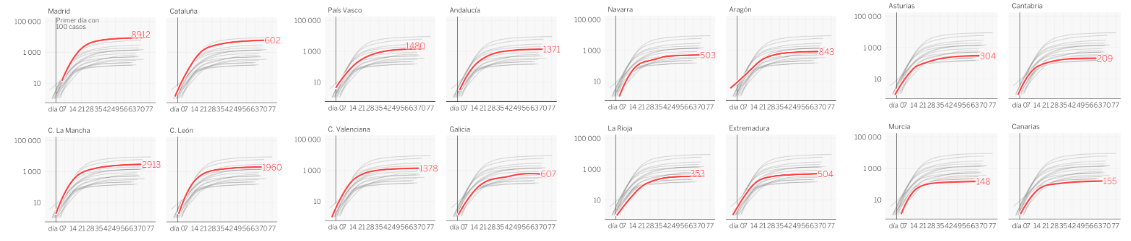
\includegraphics[width=\columnwidth]{images/introduction/covid-cases-spain.png}
    \caption{Cumulative number of death citizens in different regions of spain, from day 0 to day 77}
    \label{fig:spain-evolution-regions}
\end{figure}

In Figure \ref{fig:spain-evolution-regions} we can see the different evolution of the pandemic in the regions of the country, in terms of accumulated deaths \cite{spain-covid}. It is remarkable the unbalanced influence on the virus, with particular aggressiveness in the regions of Madrid and Catalonia.\\

Our purpose is to analyze what has been the steps that Spain has taken in order to develop different types of applications that could help with the pandemic, focusing on the most affected regions, and try to give a perspective both from a general and regional point of view.

%%%%%%%%%%%%%%%%%%%%%%%%%%

%%%%%%%% SECTION 2 %%%%%%%
\section{Review of COVID-19 applications}
\label{section:review}

In this section, it is covered the different approaches that many countries, businesses, and institutions are following for the development of applications related to the COVID-19 pandemic. On the one hand, we have exposed information and auto diagnosis applications, and on the other hand, we have explained tracking applications, focusing on explaining the two main approaches; centralized and decentralized.

\subsection{COVID-19 information and auto diagnosis solutions}
\label{subsection:information-auto-diagnosis}

Information and auto-diagnosis applications and websites are the first approaches that many regions have followed for the development of software that could help to fight the pandemic. The main aim of those software products is to offer a reliable source of information and at the same time decongest telephone lines that are offered for citizens. \\

The traditional test that can be done to a person to confirm if it is infected is the PCR test (\textit{polymerise chain reaction}), a test that can detect the presence of DNA of the virus in the patient. This method is effective, but it is really expensive at the cost of necessary chemical products, and also because the test takes a while to give a result. This caused that no country has developed more tests than 2.5\% of its' population \cite{covid19-ml}. For having a fast response, auto diagnosis applications could be an effective solution.\\

Auto diagnosis applications try to give as a result if a patient is infected with COVID-19 receiving as input some parameters that the user can introduce in a simple form. Then, those results are fed to an intelligent system, usually a machine learning model, giving as a result a binary response: if the patient is infected or not. They are not as effective as a traditional test, but they are really helpful because they produce a fast response when a patient has doubts about being infected.\\

Those applications usually ask the user to introduce parameters such as if they had a fever or if they had recently throat pain, but there have been more advanced applications like COVID-19 sounds app \cite{covid19-cambridge}, developed by Cambridge University, which asks the user to speak to the microphone, and with the sound of the voice it could determine if they are infected. \\

Although the creation of auto diagnosis applications is the first approach that many governments are following, is not the most effective way for controlling the pandemic, because their use is justified when the person present symptoms, and at that point is too late, because before presenting symptoms that person could have infected many others. Knowing that a person is infected before they present symptoms it is required to prevent the spreading of the virus, and for that other types of software are needed.

\subsection{COVID-19 tracking solutions}
\label{subsection:covid-19-tracking}

In Section \ref{subsection:information-auto-diagnosis}, we exposed the type of applications used mainly for auto diagnosis on population. This software is really useful for decongesting telephonic lines and reduce the number of visits to clinical centers, but it is not the right tool for analyzing the evolution of the pandemic and track the infected population.\\

Achieving accurate monitoring of the virus is a really difficult task, mainly due to the infectivity and for a long time that it takes to manifest the first symptoms after the patient is infected. Thankfully, the development of mobile devices and new types of connectivity offers new possibilities for tracking how the virus is disseminated in the population. \\

Security and privacy are the main concerns behind that type of technology, mainly because location and number of people that you keep contact with is information that is required to harvest from the population. Although this information is required, two approaches have been developed in recent months for the treatment of that information: centralized and decentralized approach. We are going to cover that technology in the following sections. \\

\subsubsection{Centralized approach for COVID-19 tracking}
\label{subsubsection:centralized-approach}

A Centralized approach is the most straightforward way to achieve COVID-19 contact tracing. It was first implemented in China, coinciding with the lifting of strict lockdown orders. The Chinese government is well known for using \textit{state of the art} technology for surveillance. One example of it is the usage of facial recognition techniques in order to control the activity of citizens, including targeting ethnic minorities \cite{china-massive-covid-tracking}. \\

In mid-February, when the coronavirus situation started to be less restrictive, the Chinese government implemented a scoring system, in cooperation with tech giants such as Alibaba \cite{china-massive-covid-tracking}. When a citizen wanted to use public transport or wanted to go shopping, they had to prove that they were not at risk of infecting other people. For achieving that, they had to scan a QR code before entering the place they want. This QR code was provided by the government, and when a citizen scans this code, the AliPay application gives as a result a score and a color code. When the color is green, this person is not in risk of been infected with COVID-19, when the code is yellow, the citizen is in moderated risk, finally with the color red, the citizen has a high risk of being infected, thus it would not be allowed to enter into the place \cite{china-qr-codes}. \\

There has not been a clear report on how the Chinese government calculates the score for each citizen, but, probably, that it depends mainly on user location and recent contacts that they had. This situation separates the line between government and tech giants in the Asian country and also is the perfect scenario for spreading the use of massive surveillance systems in population \cite{china-qr-codes}. \\

This approach was also followed in other Asian countries like South Korea, where the government has developed a central database that contains specific information about coronavirus cases and infections, with exact information such as detailed movements around the country, age, gender, and sex \cite{south-korea-surveillance}. This type of software gained popularity in Korea because of its tested effectiveness fighting the pandemic. \\

Although centralized solutions are more popular in Asian countries, there have been some attempts of implementations of similar systems in countries like Israel or the UK. In Israel, the government has approved an exceptional measure that allowed them to access the location of population cell phones via the network provider \cite{israel-covid-tracing}. In the case of the UK, the National Health Agency has declared that they are going to implement a centralized approach where the matches of contacts with high infection probability are going to happen in a central server \cite{uk-tracking}.\\

Centralized approaches for COVID-19 tracking are effective in societies when the government has a lot of control over the population, and where individual privacy is not widespread. But raises some concerns to be implemented in Europe or in the United States, where governments prefer to follow decentralized approaches.

\subsubsection{Decentralized approach for COVID-19 tracking}
\label{subsubsection:decentralized-approach}

The decentralized approach for COVID-19 tracking is the trend that many western countries and institutions are following. The main characteristic of decentralized methods is that they preserve the privacy of the users involved in the system, moving the tracking of the infected population from a central server to the citizen's smartphones. \\

Decentralized contact tracing is a well-known field in the literature since 2013 \cite{bell2020tracesecure}\cite{altuwaiyan2018epic}\cite{zhang2013privacy}, but during this pandemic, this work has become relevant. Also, an important breakthrough in this sense was the usage of \textit{Bluetooth Low Energy}, a variant of Bluetooth network technology that could be used to track devices which are near, without the need of using the GPS signal. \\

But it is not enough by specifying what is the technology that is going to be used for tracking the proximity between devices, it is also needed to define the protocols and algorithms that those devices are going to follow to communicate between them. In this sense, the first protocol developed was \textit{Pan-European Privacy-Preserving Proximity Tracing} (PEPP-PT) \cite{pepppt} from a collaboration between a French and a German university. This protocol combines a centralized and decentralized approach and was welcomed with enthusiasm. But, some European countries have dismissed their use because it is not as respectful of privacy as expected \cite{swiss-peppt}.\\

To solve these privacy concerns, a coalition of eight European universities have developed the protocol \textit{Decentralized Privacy-Preserving Proximity Tracing} (DP3T) \cite{dp3t-docs}, which has rapidly gained popularity in the academic and institutional field. One proof of that is the recent interest that Apple and Google are showing for following this protocol for the COVID-19 tracking application that they are developing together \cite{dp3t-google-apple}. As it is considered the new \textit{de facto} standard in coronavirus tracking, it is important to know how it works in a detailed way.\\

The DP3T protocol relies on the use of mobile devices that users are supposed to carry with them when they go to the street and have contact with people. Each mobile device should generate a unique secret key each day $t$, which is called $SK_t$. This secret key is the privacy safeguard of the user and will be the media that other devices are going to use in order to determine if they are in danger of being infected. It is important to mention also that this key is going to be finally revealed only if the user wants. \\

For generating the secret key of the day ($SK_t$), the device is going to use a public hash function $H$, which will use as a seed, the secret key of the previous day ($SK_{t-1}$). One characteristic of function $H$ is that computing the secret key for the next day ($Sk_{t+1}$) is easy having the key of the current day ($SK_t$), but it is impossible to compute the key of the previous day ($SK_{t-1}$). This is done to preserve the privacy of the user if the key of the day $t$ is revealed. \\

\begin{figure}[h]
    \centering
    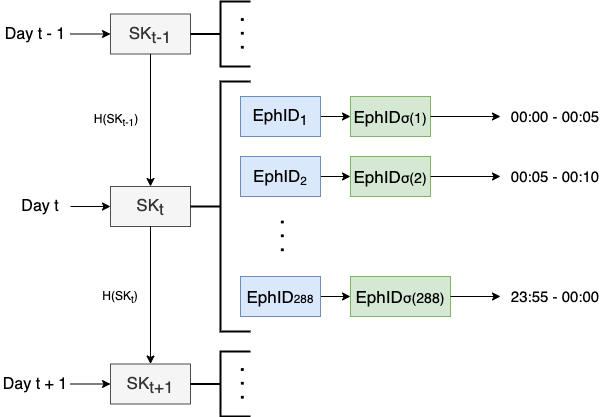
\includegraphics[scale=0.4]{images/discussion/SK-ids-diagram.png}
    \caption{Diagram of the secret key ($SK$) and ephemeral IDs ($ephID$) generated per day}
    \label{fig:sk-diagram}
\end{figure}

As shown in Figure \ref{fig:sk-diagram}, for each day $t$, mobile devices are going to generate 288 ephemeral IDs ($EphID_i$), where each ephemeral ID is going to be emitted by the devices using \textit{Bluetooth Low Energy} for 5 minutes. This is why 288 IDs are needed per day, because a day has 1440 minutes, and the IDs are only valid for 5 minutes. For the generation of the ephemeral IDs, the devices are going to use a function $G$, which is a pseudorandom generator that uses $SK_t$ as a seed (described in equation \ref{eq:ephemeral-id}).

\begin{equation}
\begin{split}
    G: SK_t \rightarrow EphID_i \\
    \{EphID_1, EphID_2, \cdots, EphID_{288}\} = \{G(SK_t), G(SK_t), \cdots, G(SK_t)\}
\end{split}
\label{eq:ephemeral-id}
\end{equation}

After the generation of the ephemeral IDs, the device should use a random permutation function ($\sigma$), to distribute the ephemeral IDs though the 288-time slots of the day (described in equation \ref{eq:ephid-permutation}). After decide which is the order of emission, the device should start to emit the identifiers.

\begin{equation}
    \begin{split}
        \sigma : \{1, \cdots, 288\} \rightarrow \{1, \cdots, 288\} \\
        \{EphID_{\sigma(1)}, EphID_{\sigma(2)}, \cdots, EphID_{\sigma(288)}\}
    \end{split}
    \label{eq:ephid-permutation}
\end{equation}

Let us suppose that during the emission, two devices are sufficiently near. Both of them are going to record the ephemeral IDs detected in a registry log. The device can not know whom the ephemeral IDs belong to, because they did not know the secret key of the day. If they would know the secret key of the day ($SK_t$) for a user, they could compute the ephemeral IDs that the device emitted in the day, because they know the function $G$. Using the ephemeral Ids logs, each device could have a registry of the contacts that it had per day, annotating also the duration and intensity of the signal detected. \\

\begin{figure}[h]
    \centering
    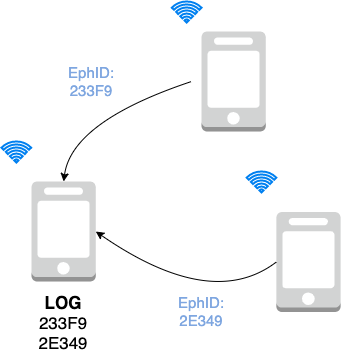
\includegraphics[scale=0.4]{images/discussion/ephid-log.png}
    \caption{When a device detects the $EphID$ of other device it adds it to a log and can not distinguish what device it came from.}
    \label{fig:ephid-log}
\end{figure}

In case that a user gets infected with COVID-19, the system has to start a process that notifies other users who have contact with the infected person and consequently starts a process of quarantine or they can contact health authorities. For starting this process, the system needs the collaboration of the local health authorities, which will determine which was the day when the person got infected (day $T$). Then, the health authorities should provide a central server that will publish the secret key of the day that the infection started ($SK_T$). Every day, all users of the system must download the list of secret keys of infected users. Having the secret key of an infected user on day $T$, each user must compute the following secret keys for each day until present day $t$, using function $H$ (Equation \ref{eq:sk-computation}).

\begin{equation}
    \begin{split}
        SK_T \\
        SK_{T+1} = H(SK_T) \\
        SK_{T+2} = H(SK_{T+1}) \\
        \cdots \\
        SK_t = H(SK_{t-1})
    \end{split}
    \label{eq:sk-computation}
\end{equation}

Having the list of secret keys, they can compute easily the ephemeral IDs of each day, using function $G$, creating a set of infected ephemeral IDs called $I$ (Equation \ref{eq:ephid-computation}).

\begin{equation}
\begin{aligned}
I ={} & \{\{G(SK_T)_1, G(SK_T)_2, \cdots, G(SK_T)_{288}\} \\
      & \cup \{G(SK_{T+1})_1, G(SK_{T+1})_2, \cdots, G(SK_{T+1})_{288}\} \\
      & \cdots \\
      & \cup \{G(SK_t)_1, G(SK_t)_2, \cdots, G(SK_t)_{288}\}\}
\end{aligned}
\label{eq:ephid-computation}
\end{equation}

Having computed the set $I$, and the logs that are locally stored in the device, it could be determined if the local user is at risk of being infected by computing the intersection between those two sets. If the intersection is empty, the user is not at risk of being infected, but if there is at least one ephemeral ID that they have in common, we can determine that the user is at risk. As we can see, the characteristics of this method allow users to know if they are infected with COVID-19, but they could not know who infected them, and also local authorities could not know how and when the citizen got infected, guaranteeing the privacy of all citizens involved.

%%%%%%%%%%%%%%%%%%%%%%%%%%

%%%%%%%% SECTION 3 %%%%%%%
\section{Discussion of COVID-19 Applications in Spain}
\label{section:discussion}

In Section \ref{section:review}, it was exposed the different types of applications that have been developed for fighting against the COVID-19 pandemic. In this section, it is going to be covered the different initiatives that have been developed in Spain, both in information applications and also in services for tracking the pandemic.

\subsection{COVID-19 Information and auto diagnosis applications in Spain}
\label{sec:information-apps-spain}

In Spain, the central source of information for the pandemic has been the website of the Ministry of Health \cite{ministerio-sanidad}. In this website is where it is published the scientific information regarding the disease, and also is where the official numbers of new infected, dead and tested population is published every day.\\

As the public health in Spain is decentralized, each autonomous community or region have all the competencies for the organization of hospitals and logistics of healthcare in the region. This has caused some of them to have developed specific applications for auto-diagnosis and also for giving specific information to the citizens of the region. In this analysis, it is covered the solutions proposed by the community of Madrid, and the community of Catalonia, the two most affected regions in the country (as shown in Figure \ref{fig:spain-evolution-regions}), and also the solution proposed by the central government.

\paragraph{CoronaMadrid} \mbox{}\\

As Madrid is the most affected region of Spain, the development of an application that could help the healthcare system to resist the pandemic was a critical task. \textit{CoronaMadrid} \cite{coronamadrid-page} was one of the first applications developed in Spain regarding the pandemic; it consists in a website and an application for Android and iOS that offers the possibility of filling a self-diagnosis form, and then a classification system would determine if you have enough significant symptoms for being considered as a COVID-19 affected. In the beginning, this application was permissive, offering the possibility of doing the diagnosis test without introducing any personal information, but nowadays this policy has changed and the user should introduce their name, personal ID, and direction in the Madrid community. This change was done to improve the reliability of the data that was collected \cite{coronamadrid-privacy}. \\

\begin{figure}[!htb]
   \begin{minipage}{0.33\textwidth}
     \centering
     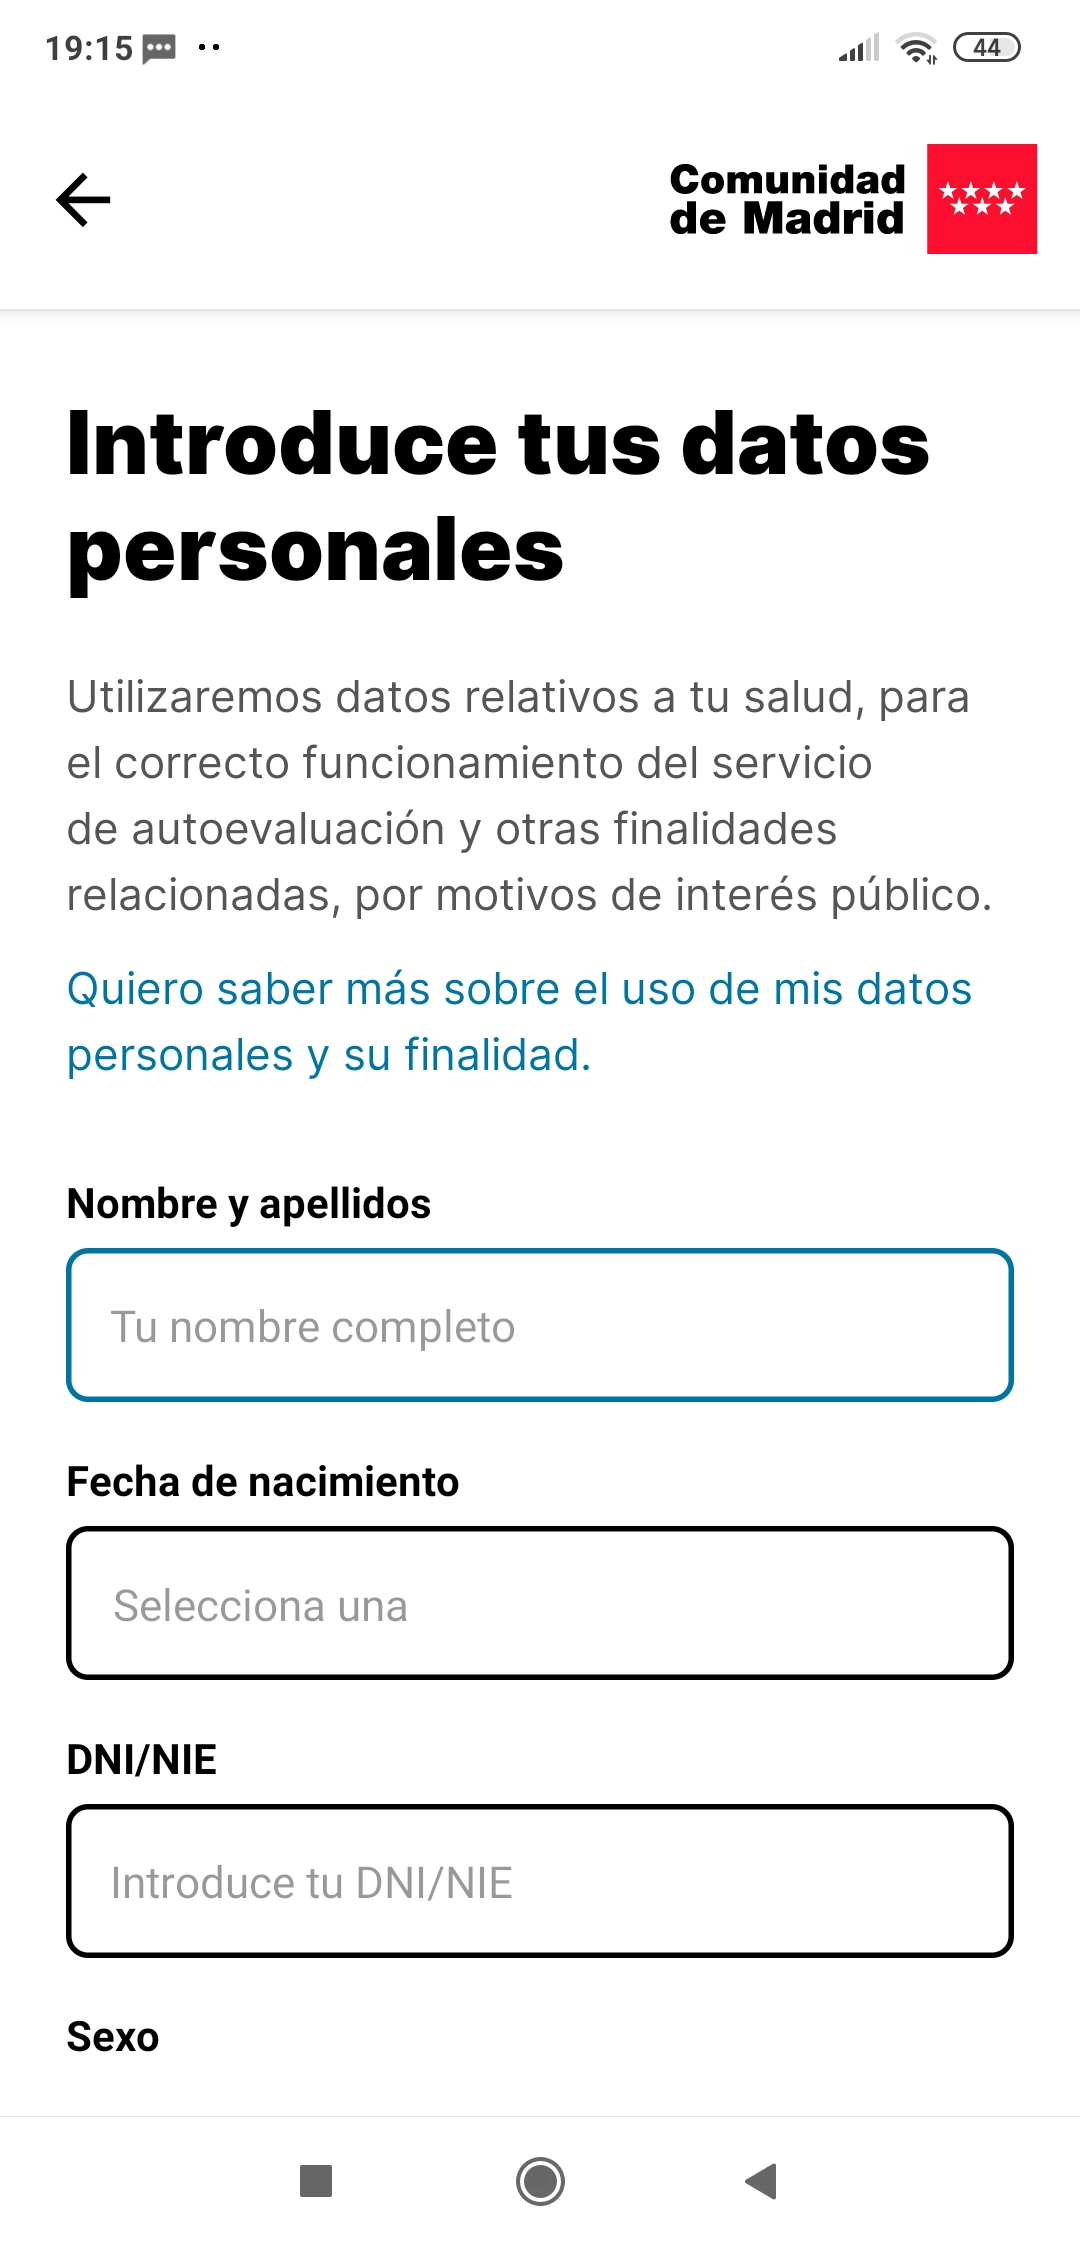
\includegraphics[scale=0.06]{images/discussion/coronamadrid-1.jpg}
   \end{minipage}\hfill
   \begin{minipage}{0.33\textwidth}
     \centering
     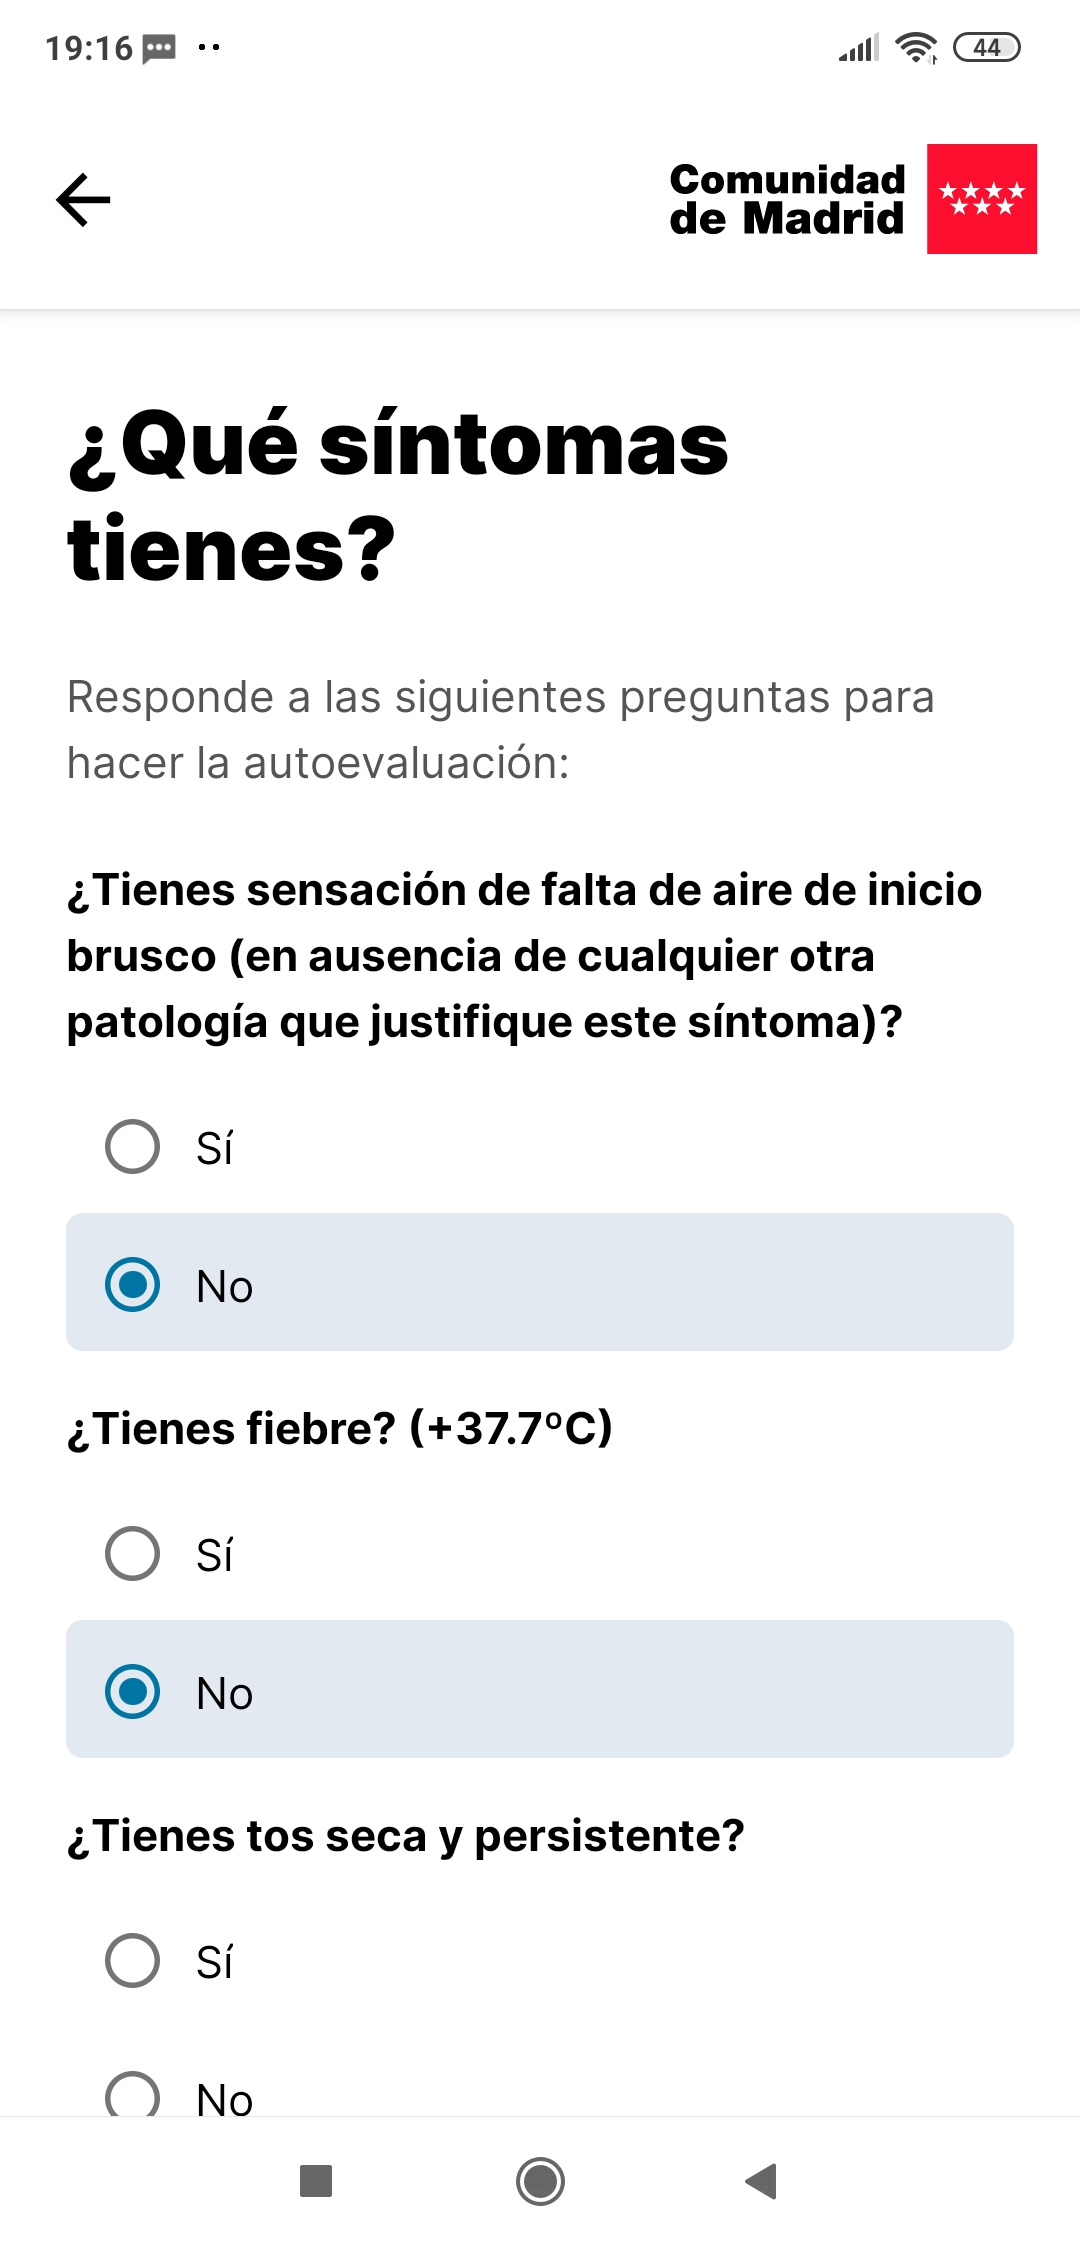
\includegraphics[scale=0.06]{images/discussion/coronamadrid-2.jpg}
   \end{minipage}
   \begin{minipage}{0.33\textwidth}
     \centering
     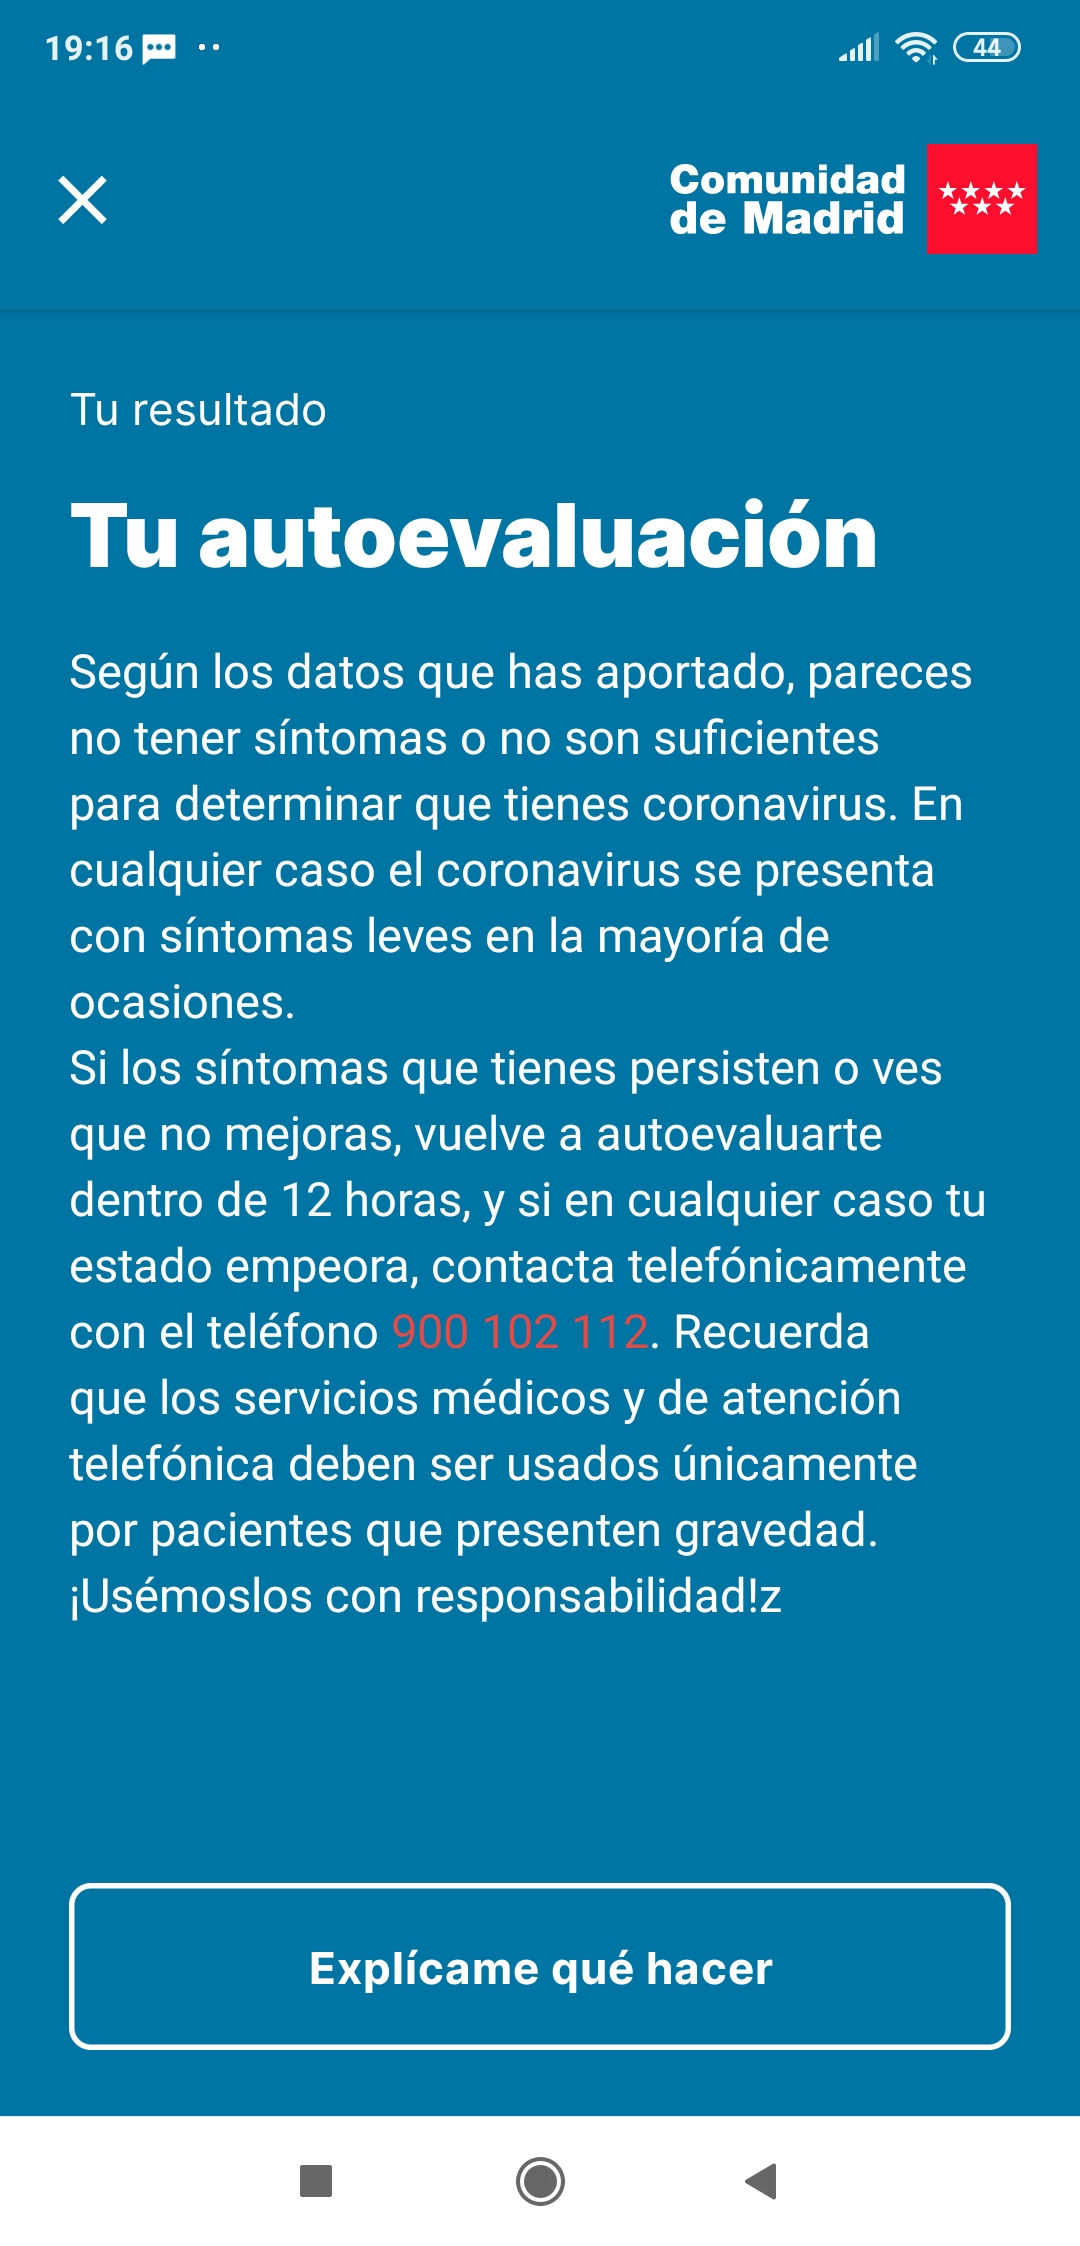
\includegraphics[scale=0.06]{images/discussion/coronamadrid-3.jpg}
   \end{minipage}
   \caption{Different screens of the application CoronaMadrid}
   \label{fig:coronamadrid}
\end{figure}

Analyzing the visual components and user experience of the application (Some screenshots of the Android app are shown in Figure \ref{fig:coronamadrid}), it consists of a simple form where the user introduces the personal details in the beginning, and then answer several questions successively in each screen. After that process, the application gives a result, showing the actuation protocol in case it is needed. The application is characterized by its simplicity, which makes it accessible for all types of users.

\paragraph{STOP COVID19 CAT} \mbox{} \\

It is also remarkable the impact of the COVID-19 pandemic in the region of Catalonia, being the second community in the number of deaths and total infected population. This situation pushed this community to follow Madrid in the development of an information application \cite{first-covid19-apps}, centered on the Catalonia region. The name of the application is STOP COVID19 CAT \cite{stop-covid19-cat}, and it was developed by the Generalitat de Catalunya (Government of Catalonia). The operation of the application is very similar to \textit{CoronaMadrid}, with a specific form which performs an auto-diagnosis test. In the field of data consistency, the main difference between them is that this application asks for the ID number of the sanitary card, and did not ask for the direction within the community, which is directly obtained from the GPS of the device. \\

\begin{figure}[!htb]
   \begin{minipage}{0.33\textwidth}
     \centering
     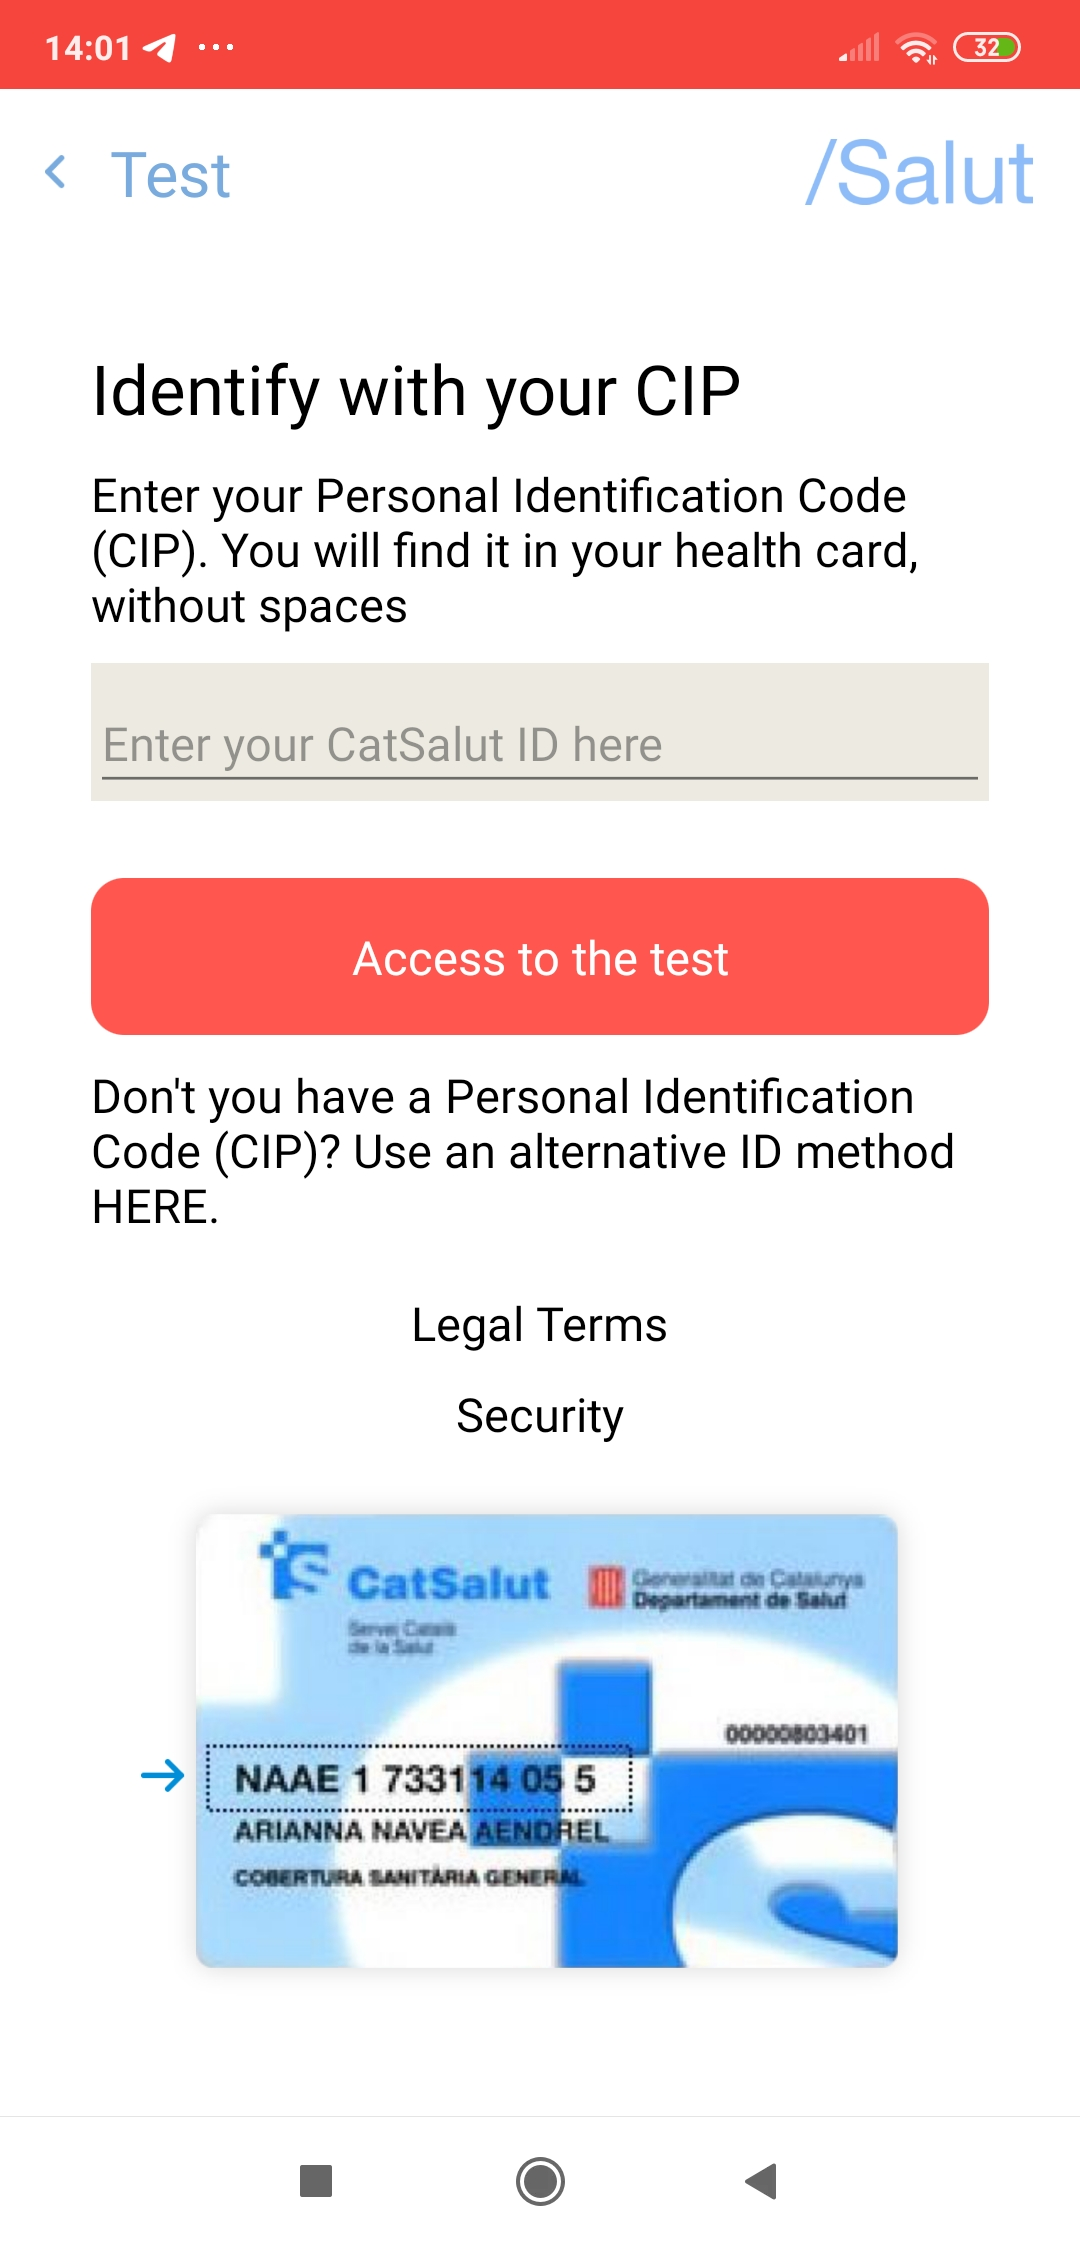
\includegraphics[scale=0.06]{images/discussion/covid-cat-1.jpg}
   \end{minipage}\hfill
   \begin{minipage}{0.33\textwidth}
     \centering
     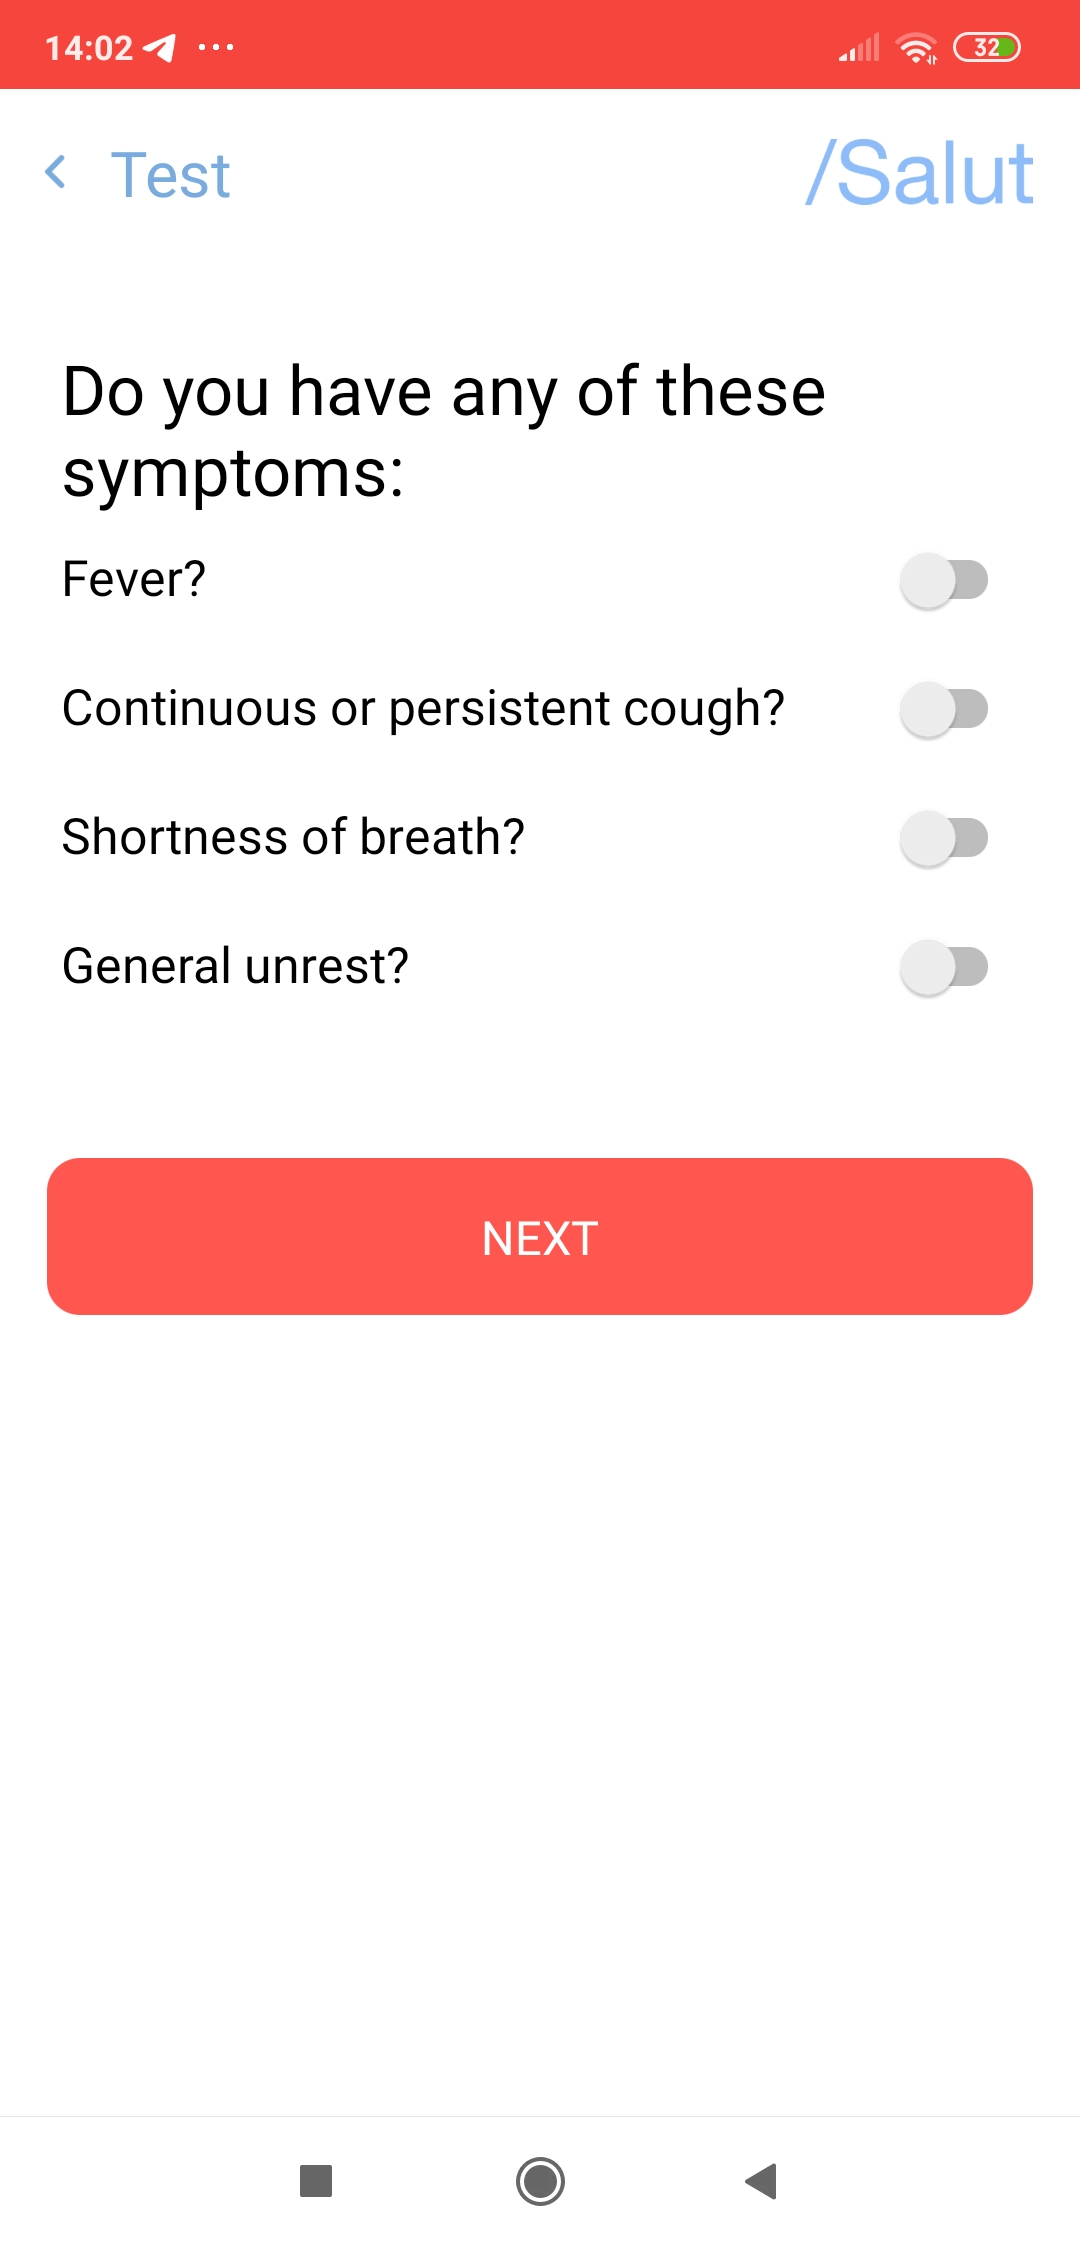
\includegraphics[scale=0.06]{images/discussion/covid-cat-2.jpg}
   \end{minipage}
   \begin{minipage}{0.33\textwidth}
     \centering
     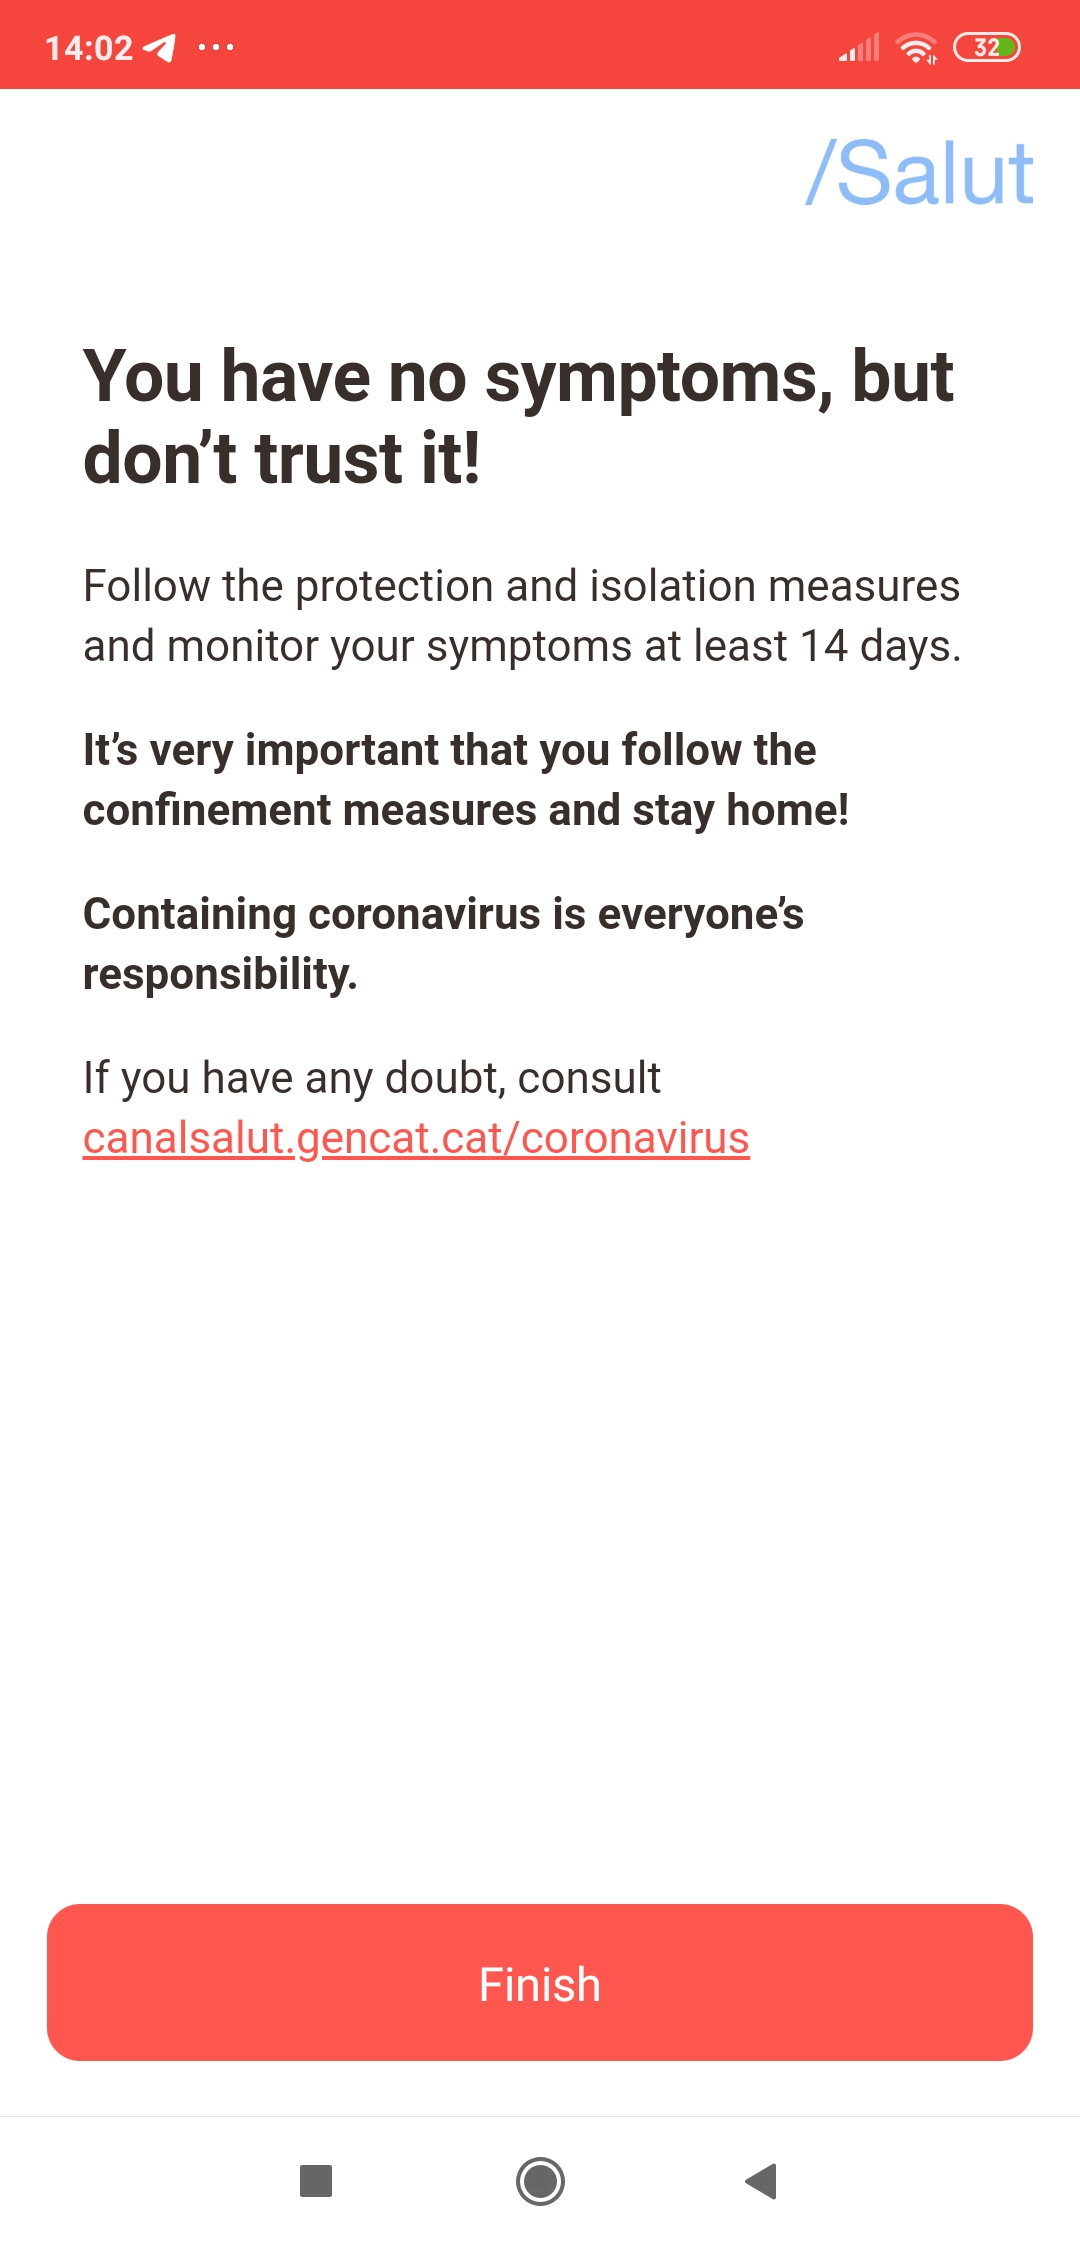
\includegraphics[scale=0.06]{images/discussion/covid-cat-3.jpg}
   \end{minipage}
   \caption{Different screens of the application STOP COVID19 CAT}
   \label{fig:covid-cat}
\end{figure}

Speaking about user experience, STOP COVID19 CAT has a worse performance. The display of the information is less intuitive, mainly because of the use of switches instead of radio buttons, as shown in Figure \ref{fig:covid-cat}. Another significant difference is that the Catalonia app allows us to do as many auto evaluations as we want, and \textit{CoronaMadrid} only allows users to do the evaluation once per day. This control over the frequency improves the reliability of the data collected. 

\paragraph{Asistencia COVID-19} \mbox{} \\

As \textit{CoronaMadrid} was the first auto diagnosis application of the virus in Spain, when the government wanted to do a central version that will be used as a substitute for the ones developed in the autonomous communities, the logic path will be to copy the main functionalities of it. The application developed by the National Department of digitization and artificial intelligence (\textit{Secretaría de Estado de digitalización e inteligencia artificial} in Spanish), was called Asistencia COVID-19. The way that these application works is really similar in how \textit{CoronaMadrid} works, especially in the data that is recollected: name, national ID number, direction, and autonomous community where you are located. Also, it requires the activation of the GPS service in the device, which has caused some social controversy \cite{geolocalization-asistencia-covid-19}. It is important to mention that the operability of this application is limited to some regions, initially it was developed for Madrid, but now it has been extended to five additional communities.\\

\begin{figure}[!htb]
   \begin{minipage}{0.33\textwidth}
     \centering
     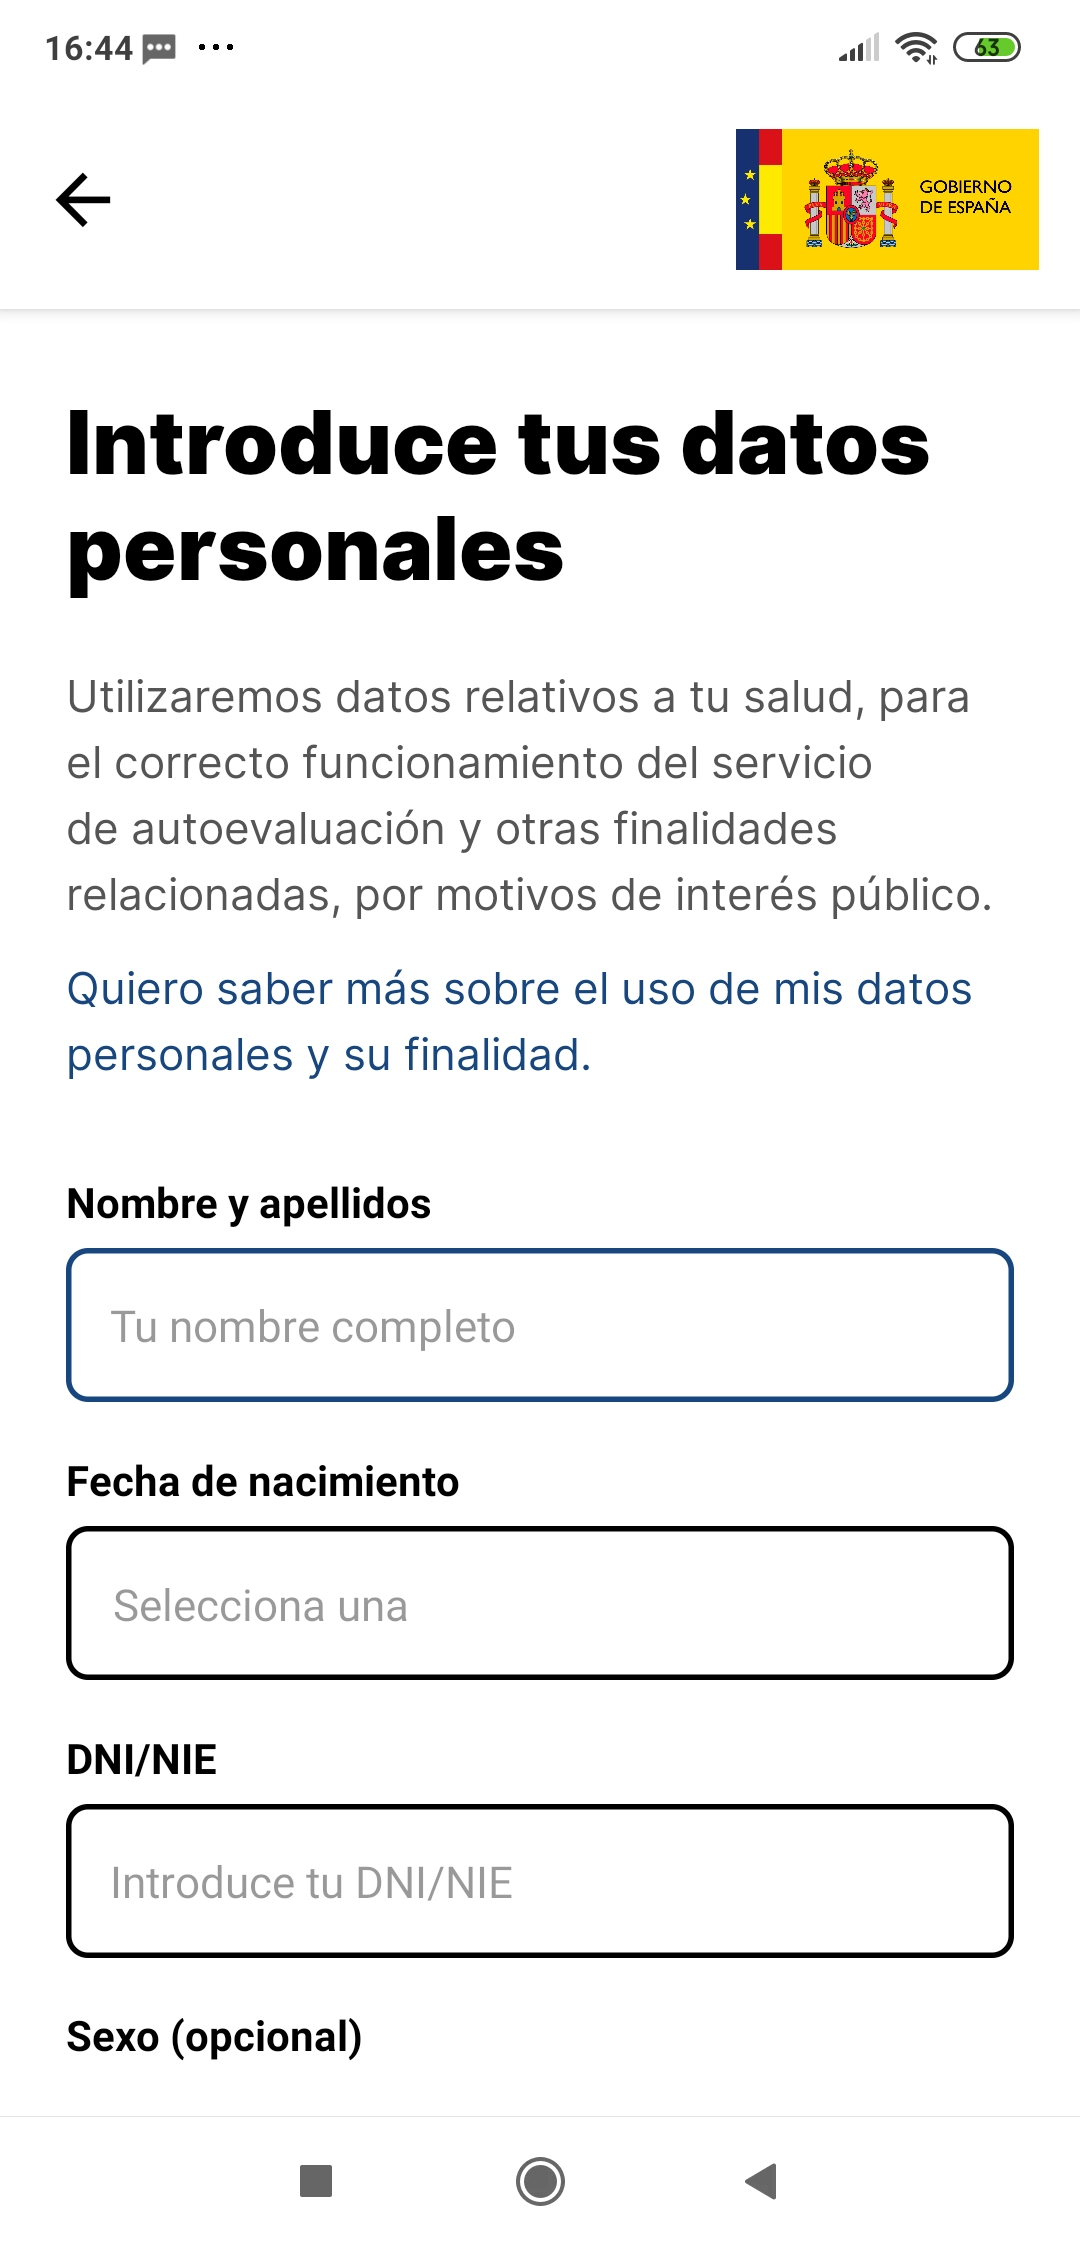
\includegraphics[scale=0.06]{images/discussion/asistencia-covid-1.jpg}
   \end{minipage}\hfill
   \begin{minipage}{0.33\textwidth}
     \centering
     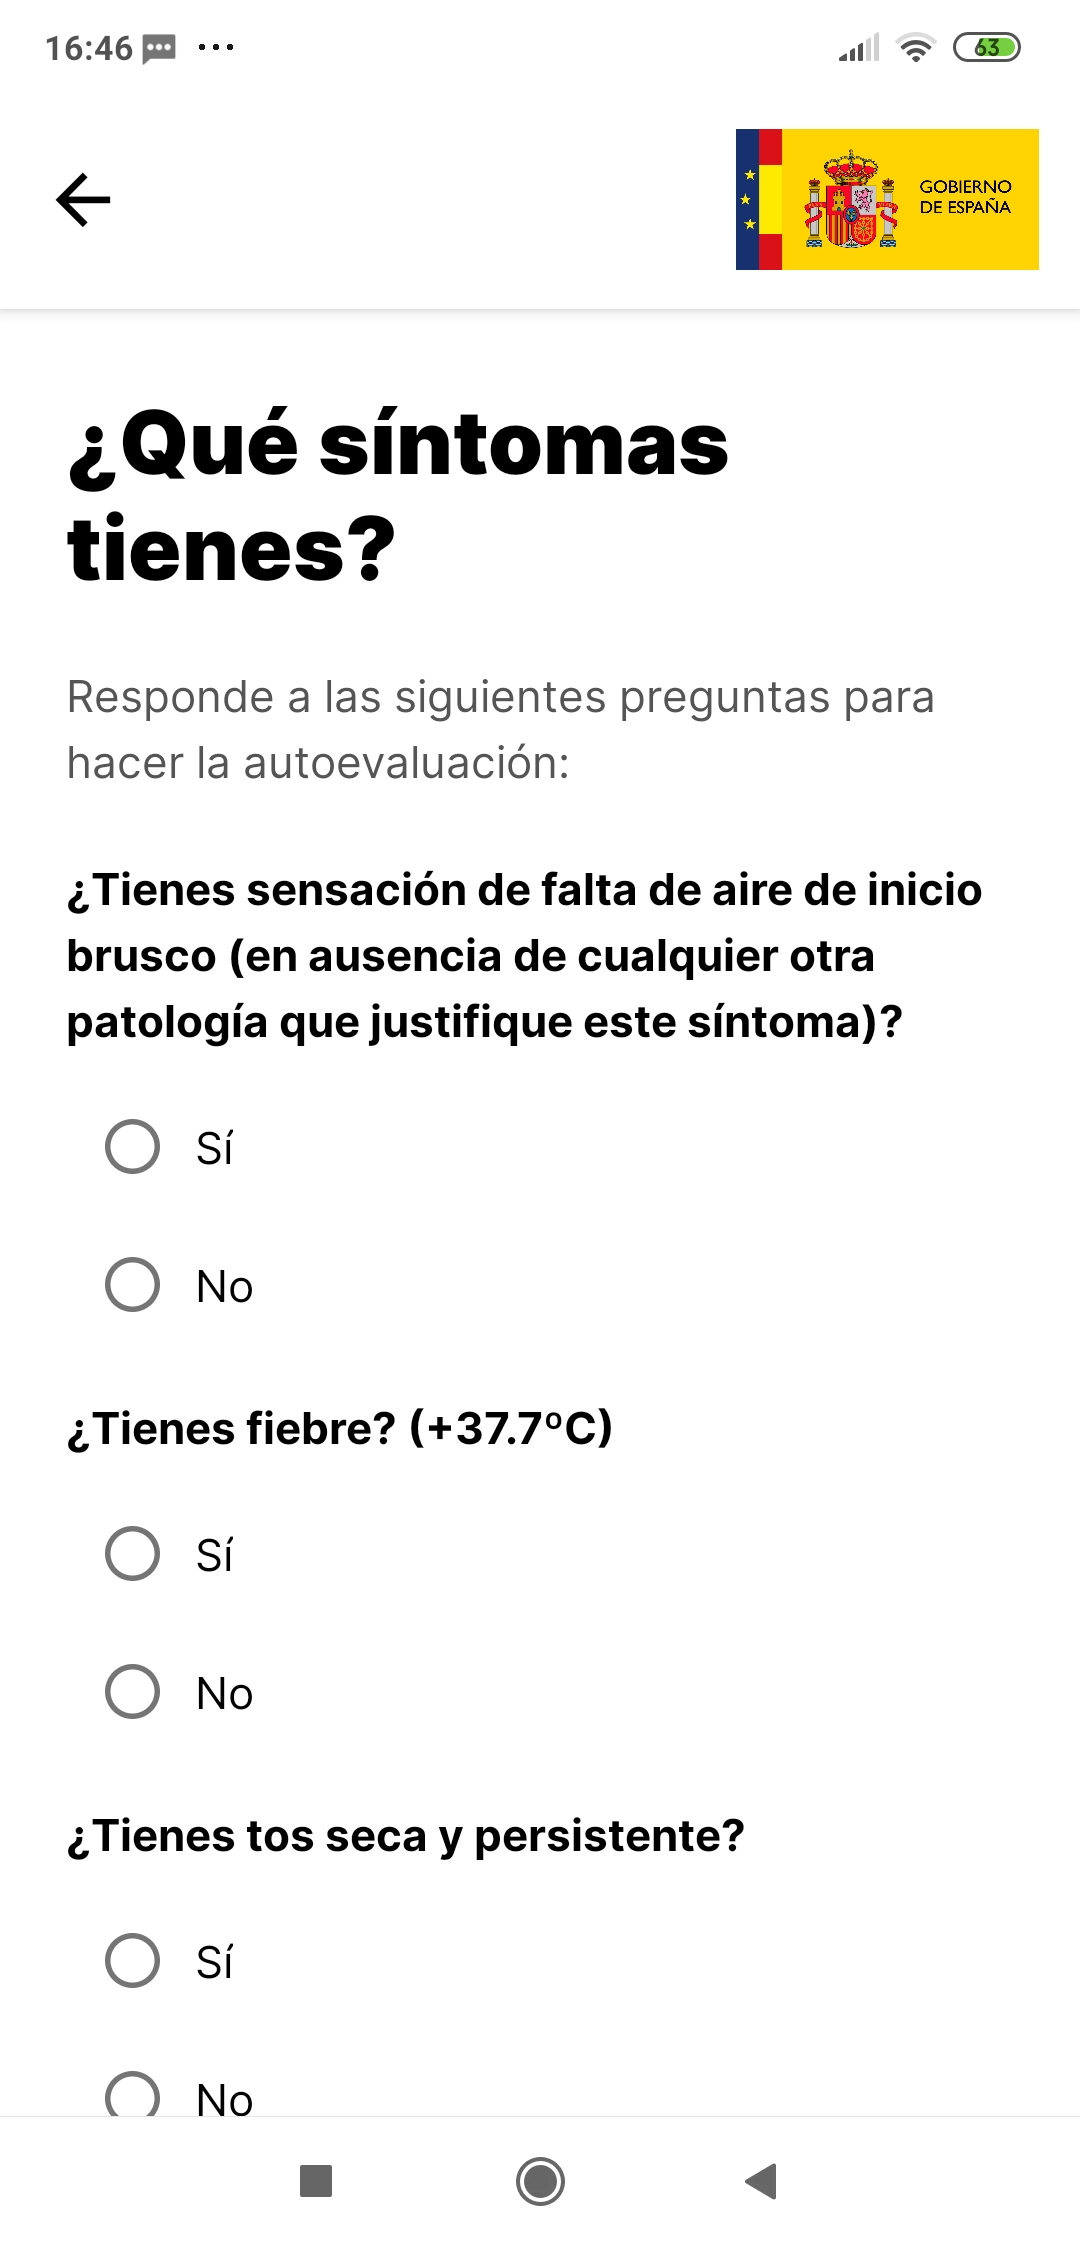
\includegraphics[scale=0.06]{images/discussion/asistencia-covid-2.jpg}
   \end{minipage}
   \begin{minipage}{0.33\textwidth}
     \centering
     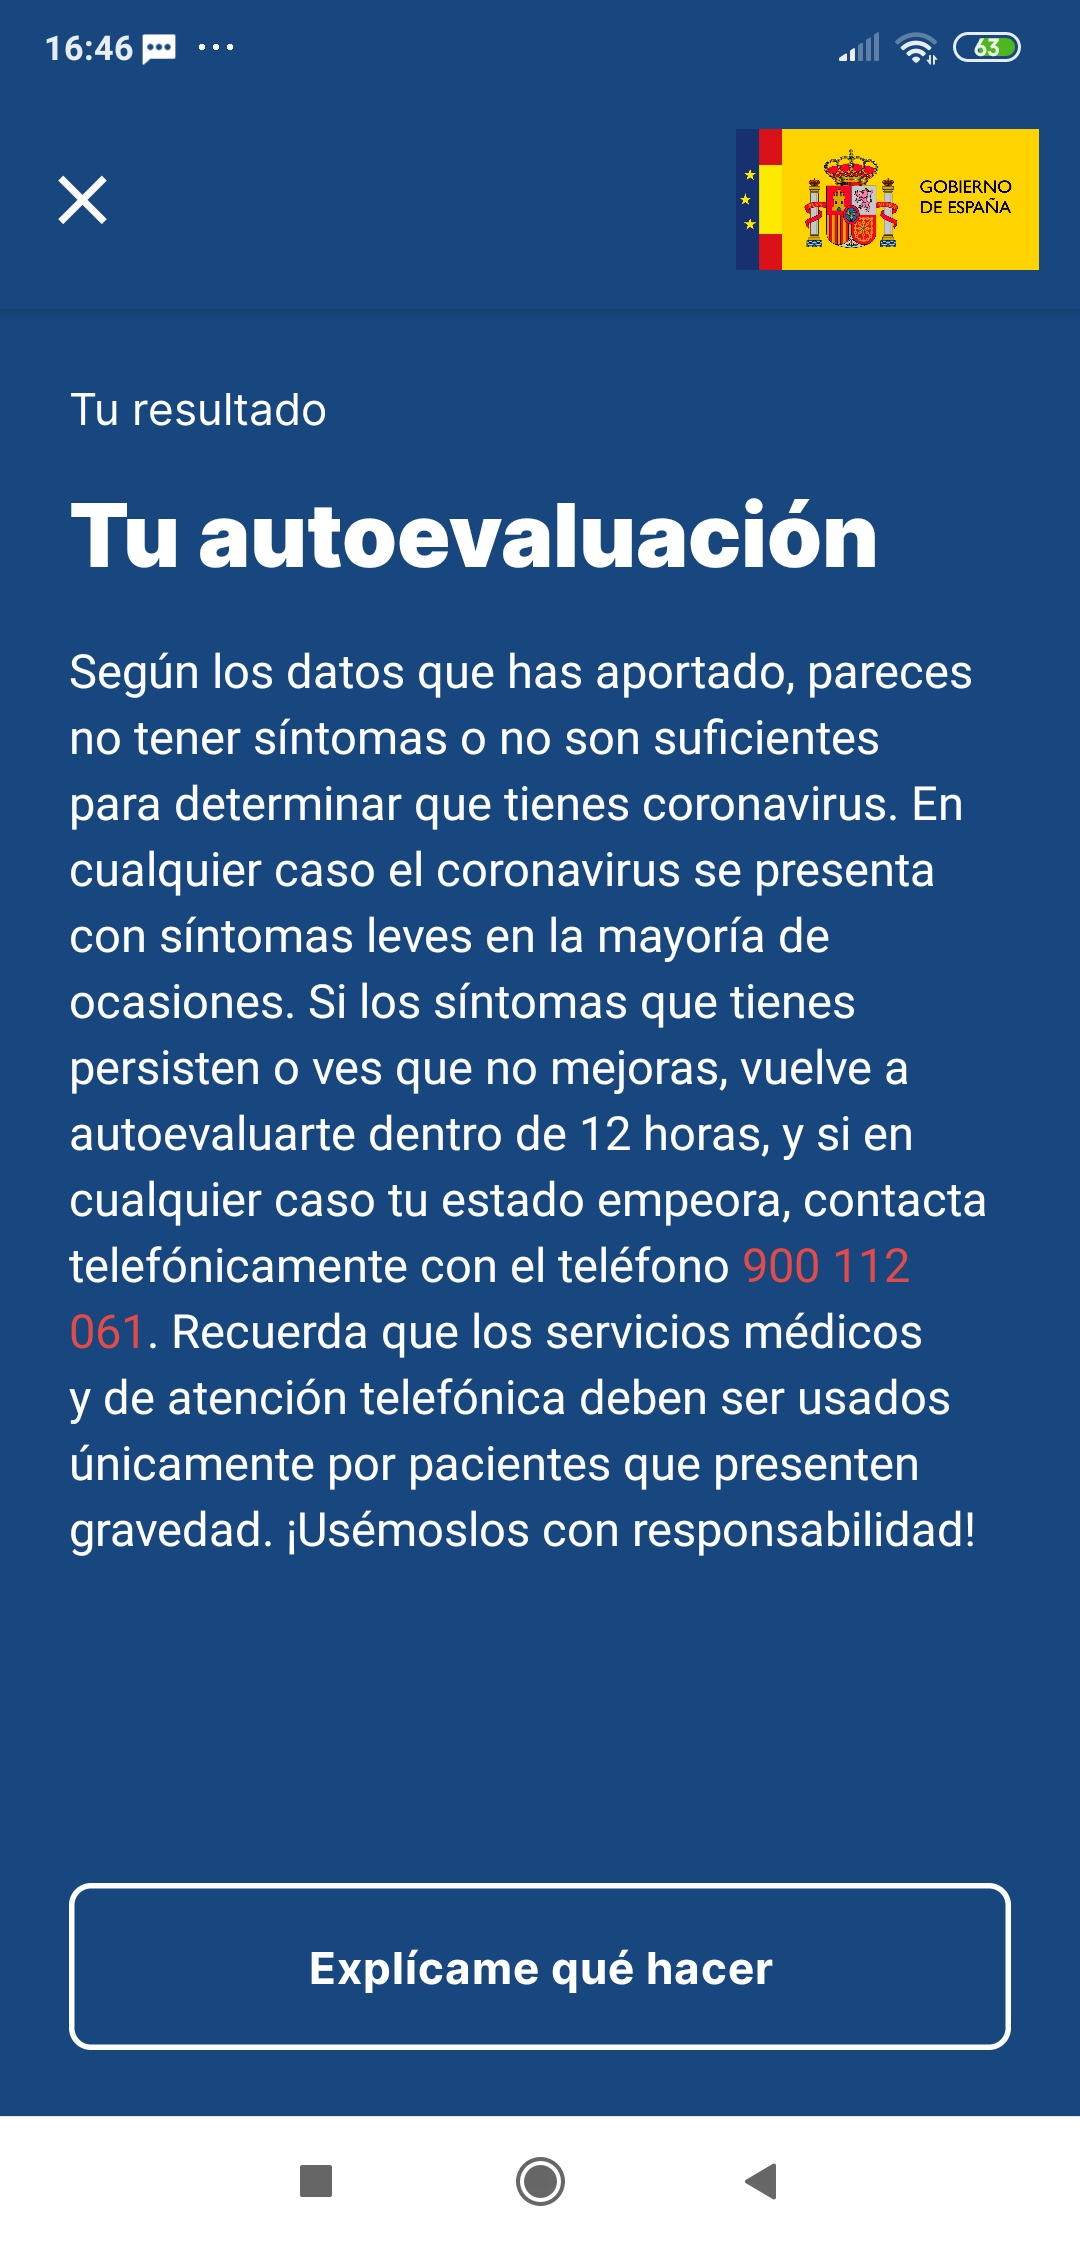
\includegraphics[scale=0.06]{images/discussion/asistencia-covid-3.jpg}
   \end{minipage}
   \caption{Different screens of the application Asistencia COVID-19}
   \label{fig:asistencia-covid-19}
\end{figure}

The analysis of the user interface of the application makes clear that it was inspired by \textit{CoronaMadrid}, (similarities in the user interface can be shown in Figure \ref{fig:asistencia-covid-19}). One visual element that hold important similarities between those apps are forms, having essentially the same information, with some minor differences; especially in the one for introducing personal details.

\subsection{COVID-19 tracking solutions in Spain}
\label{sec:information-apps-spain}

As it was discussed in Section \ref{section:review}, the most effective software tool for fighting against the evolution of the pandemic in a region is by using a tracking application. In Spain, there have not been many movements in that direction, because they have mainly centered the efforts in the development of information and auto diagnosis applications.\\

Recent moves towards the direction of the creation of a COVID-19 tracking application, points out to the use of a decentralized approach (reviewed on Section \ref{subsubsection:decentralized-approach}), using the Barcelona Supercomputing Center (BSC) as the central server for the processing of all the data generated \cite{covid19-tracking-bsc}. Also, the government is considering the possibility of using the Apple and Google system, which provides a public API (\textit{Application Programming Interface}), from which they can build their own system \cite{covid19-apple-google}.\\

This application is going to be developed by the National Department of digitization and artificial intelligence, the same team that previously developed Asistencia COVID-19 (Section \ref{sec:information-apps-spain}). The application is estimated to be launched in June, where the intention is to start testing the application in a more controlled environment, like the Canary Islands \cite{covid19-canary}. The collaboration between the government of the islands and the central government is key to achieve the successful implantation of the application. \\

%%%%%%%%%%%%%%%%%%%%%%%%%%

%%%%%%%% SECTION 4 %%%%%%%
\section{Conclusions}
\label{section:conclusions}

In this work, we reviewed the current approaches for building applications that could help society to fight against the COVID-19 pandemic.\\

In Section \ref{section:review} we saw that the most straightforward path for building software products is by creating information and auto diagnosis applications. We can confirm that they are simple, but there is significant room for improvement. Mainly because they are based on machine learning models that expects some parameters as input. If the applications can introduce more precise parameters to those models, we can expect more precise results from them. Also, it is relevant the information part of those applications, because in this times there has been a significant spread of fake news, mainly related to the scientific information about the virus (for example, there has been fake news about how the virus is affected by high temperatures), and offering a scientifically verified source of information that citizens can consult is a crucial task.\\

When analyzing tracking applications we can confirm that the main issue about them is privacy. A centralized approach could be effective but it is not respectful of individual rights, furthermore, in countries where it has been developed they did not reveal their sources of information. This is why several countries and institutions prefer decentralized approaches, although they are more difficult to implement. In theory, they are more respectful of privacy, but the concrete implementation of them is also relevant and for sure it would be needed a privacy consultancy when a stable implementation came into the market. \\

Finally, it was discussed in Section \ref{section:discussion} how the position of Spain was in this field. The decentralized nature of the healthcare system was a disadvantage in this sense because all efforts for creating applications were disseminated thought the autonomous communities. As it is more simple, regions focused on the development of information applications and that caused that many of them do not have the expected adoption by the population. During the month of May is where the development of a tracking application came into public discussion, but it is difficult to coordinate their use around all the territory of the country. We can conclude that the efforts of the Spanish government go in a good direction, with the focus on a decentralized tracking approach, but there is still a lot of work to do.

%%%%%%%%%%%%%%%%%%%%%%%%%%

\newpage{\pagestyle{empty}}

%%%%%% BIBLIOGRAPHY %%%%%%
\addcontentsline{toc}{section}{References}

\bibliographystyle{acm}
\bibliography{bibliography}
\nocite{*}
%%%%%%%%%%%%%%%%%%%%%%%%%

\end{document}